<![CDATA[% --- Unified Chapter on Benin Specificities ---
\chapter{Caractéristiques du Trafic Routier au Bénin : Contexte, Infrastructures, Comportements et Défis de Modélisation}
\label{chap:specificites_benin}

% Optional Introduction (Can be refined)
Ce chapitre présente les caractéristiques uniques du trafic routier au Bénin, en mettant l'accent sur le contexte socio-économique, l'état des infrastructures, la composition du parc automobile dominé par les motos, leurs comportements spécifiques, et les défis qui en découlent pour la modélisation mathématique.

\section{Contexte Socio-Économique et Défis du Transport}
\label{sec:contexte_socio_economique}

Le Bénin, comme de nombreux pays d'Afrique de l'Ouest, connaît une urbanisation rapide et une croissance démographique soutenue. Selon l'Institut National de la Statistique et de l'Analyse Économique (INSAE), la population urbaine du Bénin représentait environ 48\% de la population totale en 2019, avec une concentration particulière dans les villes de Cotonou, Porto-Novo et Parakou.

Cette urbanisation s'accompagne d'une demande croissante en mobilité, dans un contexte où les infrastructures peinent à suivre le rythme de développement. Selon la Banque Mondiale \cite{worldbank2019benin}, le Bénin doit faire face à plusieurs défis majeurs dans le secteur des transports :

\begin{itemize}
    \item Un \textbf{réseau routier insuffisant et en mauvais état}, avec seulement 30\% des routes nationales en bon état;
    \item Une \textbf{motorisation croissante}, particulièrement celle des deux-roues motorisés, qui échappe en grande partie aux réglementations;
    \item Un \textbf{système de transport public formel quasi inexistant}, remplacé par des services informels;
    \item Une \textbf{gestion urbaine limitée}, avec peu de planification intégrée transport-urbanisme.
\end{itemize}

Ces défis ont conduit à l'émergence d'un système de transport dominé par des solutions adaptatives, parmi lesquelles les motos-taxis (communément appelées \textbf{Zémidjans}) occupent une place prépondérante, constituant un service de transport public informel mais essentiel.

\section{Le Réseau Routier Béninois}
\label{sec:reseau_routier_beninois}

Le réseau routier béninois présente une grande hétérogénéité qui impacte significativement la dynamique du trafic.

\subsection{Hétérogénéité des Infrastructures Routières}
\label{subsec:heterogeneite_infra}

Selon les données de la Banque Mondiale \cite{worldbank2019benin}, le réseau routier béninois totalise environ 18 500 km, dont seulement 9,7\% (1 800 km) sont pavés à l'échelle nationale. Cette proportion varie significativement entre les zones rurales et urbaines. On distingue quatre principales catégories de revêtement, chacune influençant différemment la circulation :

\begin{itemize}
    \item \textbf{Routes bitumées} : Principalement dans les grandes villes et sur les axes majeurs (jusqu'à 30-35\% du réseau urbain à Cotonou). Leur qualité varie de bien entretenues à fortement dégradées (nids-de-poule).
    \item \textbf{Routes en terre ou latérite} : Majoritaires (environ 30\% du réseau urbain, majorité du rural), sensibles au climat (poussière en saison sèche, boue en saison des pluies), souvent difficilement praticables pour les voitures mais accessibles aux motos.
    \item \textbf{Routes pavées} : Dans certaines zones urbaines/périurbaines (environ 10\% du réseau urbain), bonne adhérence mais vibrations ralentissant les voitures plus que les motos.
    \item \textbf{Pistes et voies informelles} : Créées par l'usage, souvent inaccessibles aux voitures mais empruntées par les motos (réseau parallèle).
\end{itemize}

\begin{figure}[htbp]
    \centering
    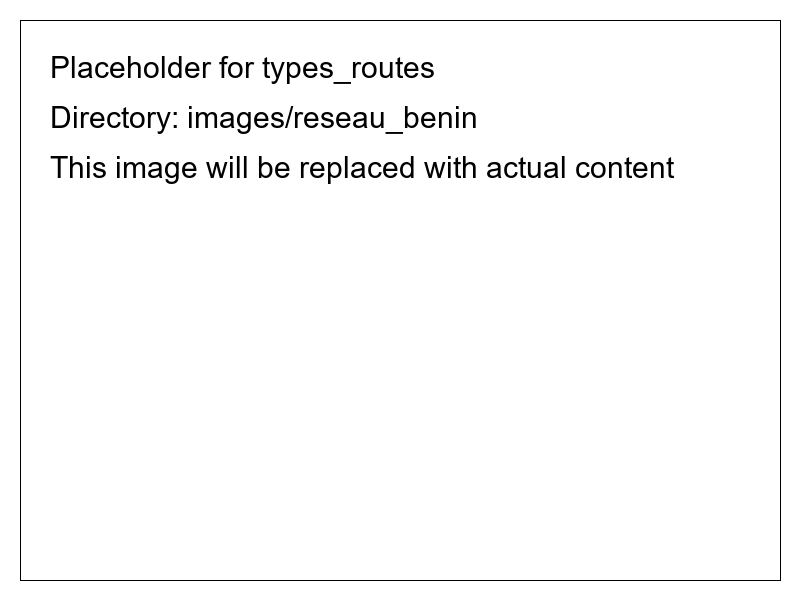
\includegraphics[width=0.9\textwidth]{images/reseau_benin/types_routes} % Assuming this image exists and is correct
    \caption{Les différents types de routes au Bénin : (a) route bitumée à Cotonou; (b) route en terre en zone périurbaine; (c) route pavée; (d) piste accessible uniquement aux motos.}
    \label{fig:types_routes} % Kept original label
\end{figure}

\begin{remark}
Cette diversité des revêtements affecte différemment chaque classe de véhicule. Notamment, les motos sont nettement moins affectées que les voitures par la dégradation de la chaussée, ce qui renforce leur avantage comparatif et nécessitera une prise en compte spécifique dans la modélisation.
\end{remark}

\subsection{Organisation Spatiale du Réseau}
\label{subsec:organisation_spatiale} % Kept original label

La configuration du réseau présente plusieurs particularités structurelles :
\begin{itemize}
    \item \textbf{Structure radiale} dans les grandes villes (ex: Cotonou), créant des points de congestion centraux.
    \item \textbf{Voies à largeur variable}, créant des goulots d'étranglement affectant moins les motos.
    \item \textbf{Rareté des voies rapides dédiées}, limitant la séparation des flux par vitesse.
    \item \textbf{Zones d'habitat spontané} avec réseaux irréguliers où coexistent véhicules et piétons, forte présence de motos.
\end{itemize}

\subsection{Gestion des Intersections et Régulation du Trafic}
\label{subsec:gestion_intersections_regulation}

La régulation et la gestion des intersections au Bénin présentent des spécificités qui complexifient leur modélisation :
\begin{itemize}
    \item \textbf{Faible densité de feux de signalisation} : Moins de 20\% des intersections urbaines sont régulées par des feux, souvent sujets à des pannes \cite{loggoh2019traffic}. Ils sont concentrés dans les centres-villes.
    \item \textbf{Ronds-points surchargés} : Souvent non régulés, ils constituent des points de congestion majeurs.
    \item \textbf{Présence d'agents de circulation} aux carrefours majeurs, introduisant une variabilité humaine.
    \item \textbf{Règles de priorité souvent négociées} de manière informelle entre usagers, particulièrement aux intersections non régulées.
    \item \textbf{Respect variable du code de la route}, avec une tolérance particulière pour les comportements des conducteurs de motos.
\end{itemize}
Ces caractéristiques créent un environnement routier où la négociation et l'adaptabilité priment souvent sur le respect strict des règles formelles.

\begin{figure}[htbp]
    \centering
    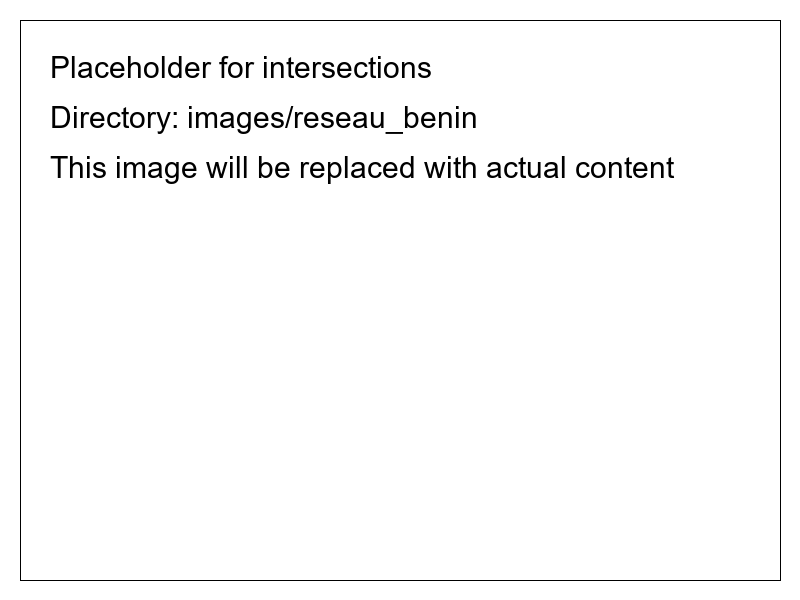
\includegraphics[width=0.8\textwidth]{images/reseau_benin/intersections} % Assuming this image exists and is correct
    \caption{Gestion des intersections au Bénin : (a) carrefour sans feux avec agent de circulation; (b) rond-point congestionné; (c) intersection non régulée avec motos prédominantes.}
    \label{fig:intersections} % Kept original label
\end{figure}

% Theorem environment might be better placed in the modeling chapter, but kept here for now as in original
\begin{theorem}[Modélisation des intersections béninoises]
Dans notre modèle, une intersection sera représentée par un terme source/puits $S_i(x,t)$ dans l'équation de conservation, avec :
\begin{align}
S_i (x,t) = \alpha_i (t) \cdot \delta(x-x_0)
\end{align}
où $\alpha_i(t)$ représente le flux entrant/sortant de véhicules de classe $i$, $\delta$ est la distribution de Dirac, et $x_0$ la position de l'intersection.
\end{theorem}

\section{Composition Hétérogène du Parc Automobile}
\label{sec:composition_parc}

Le parc automobile béninois présente une structure très différente de celle des pays occidentaux, caractérisée par une grande diversité et une prédominance marquée des deux-roues motorisés. Selon les études disponibles, notamment celle de l'AERC \cite{aerc2019taxi}, la composition approximative du trafic dans les principales villes est :

\begin{itemize}
    \item \textbf{Motos et tricycles} : Représentant 70-80\% des véhicules en circulation, elles constituent l'épine dorsale du transport urbain. On distingue les motos privées et les Zémidjans (motos-taxis).
    \item \textbf{Voitures particulières} : Environ 10-15\% du parc, souvent importées d'occasion.
    \item \textbf{Taxis-voitures} (généralement jaunes) : Environ 5-8\% du parc urbain.
    \item \textbf{Minibus et bus} : Transport en commun, environ 2-3\%.
    \item \textbf{Camions et poids lourds} : Environ 3-7\%, principalement sur les axes interurbains et zones portuaires.
\end{itemize}

% Include the table if it adds value beyond the list
\begin{table}[htbp]
    \centering
    \caption{Paramètres caractéristiques (indicatifs) par classe de véhicule} % Adjusted caption
    \label{tab:parametres_vehicules} % Kept original label
    \begin{tabular}{lcccc}
        \toprule
        \textbf{Classe} & \textbf{$v_{i,\max}^0$ (km/h)} & \textbf{$\rho_{i,\max}$ (véh/km)} & \textbf{Coefficient $\mu_i$} & \textbf{Impact relatif} \\
         & & & & \textbf{du type de route} \\
        \midrule
        Motos & 60 & 240 & -- & 1.0 \\
        Voitures & 70 & 180 & 0.3 & 0.7 \\
        Taxis & 65 & 180 & 0.4 & 0.8 \\
        Bus & 55 & 140 & 0.5 & 0.6 \\
        Camions & 50 & 120 & 0.6 & 0.5 \\
        \bottomrule
    \end{tabular}
\end{table}
% Note: The values in this table should be verified/sourced appropriately in the final document.

\section{Rôle Central et Comportements Spécifiques des Motos}
\label{sec:comportements_motos}

Les motos jouent un rôle central et adoptent des comportements de conduite spécifiques qui les distinguent nettement des autres usagers et influencent profondément la dynamique du trafic. Ces comportements révèlent une forme d'auto-organisation adaptative \cite{loggoh2019traffic, aerc2019taxi}.

\subsection{Pratiques de Conduite Distinctives}
\label{subsec:pratiques_conduite}

\subsubsection{Gap-Filling (Remplissage des Espaces)}
\label{subsubsec:gap_filling}
Le \textit{gap-filling} désigne la tendance des motos à utiliser tous les espaces disponibles entre les véhicules plus grands \cite{fan2013heterogeneous, kumar2018motorcycle}.
\begin{itemize}
    \item Utilisation systématique des espaces inter-files, même réduits (<1m).
    \item Formation de files virtuelles supplémentaires (jusqu'à 4-5 observées sur 2 voies).
    \item Optimisation dynamique de l'espace.
    \item Maintien d'une vitesse souvent supérieure à celle des autres véhicules en congestion légère/modérée.
\end{itemize}

\subsubsection{Interweaving (Circulation en Zigzag)}
\label{subsubsec:interweaving}
L'\textit{interweaving} désigne la pratique consistant à se faufiler entre les véhicules en changeant fréquemment de trajectoire \cite{kumar2018motorcycle}.
\begin{itemize}
    \item Changements de direction rapides et fréquents (7.3/km obs. vs 0.8/km pour voitures).
    \item Anticipation très courte, décisions en temps réel.
    \item Utilisation d'espaces temporaires entre véhicules en mouvement.
    \item Forte tolérance au risque, marges de sécurité réduites.
\end{itemize}

\subsubsection{Front-Loading aux Intersections}
\label{subsubsec:front_loading}
Le \textit{front-loading} désigne l'accumulation préférentielle des motos à l'avant des files d'attente aux intersections (feux rouges).
\begin{itemize}
    \item Filtrage systématique vers l'avant de la file.
    \item Occupation de tout l'espace devant la ligne d'arrêt.
    \item Anticipation du démarrage avant le passage au vert.
    \item Accélération rapide dégageant l'intersection plus vite.
\end{itemize}
Ce phénomène crée une ségrégation spontanée des classes de véhicules aux intersections.

\subsubsection{Adaptation aux Infrastructures}
\label{subsubsec:adaptation_infra}
Les motos peuvent maintenir une vitesse relativement élevée sur des surfaces où les voitures doivent considérablement ralentir (routes dégradées, en terre) \cite{karthik2019estimation}. Elles utilisent également les pistes et voies informelles inaccessibles aux autres véhicules.

\begin{figure}[htbp]
    \centering
    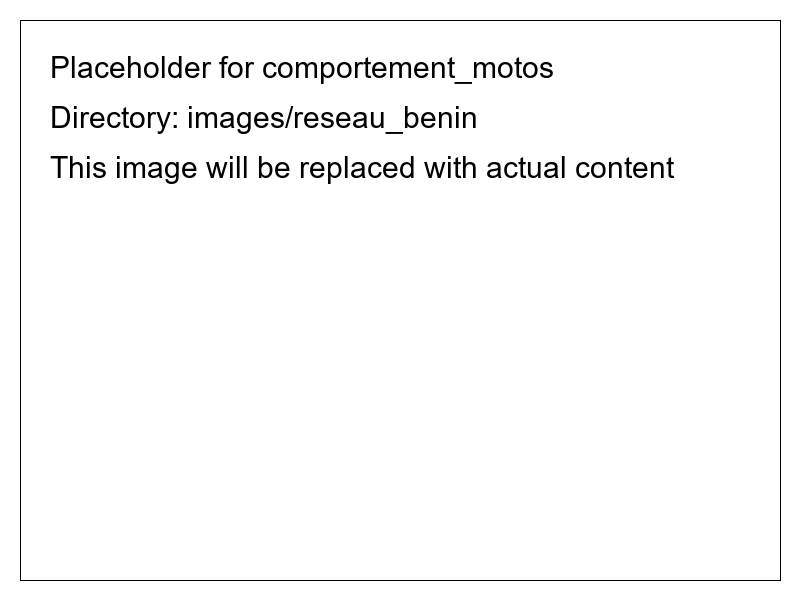
\includegraphics[width=0.9\textwidth]{images/reseau_benin/comportement_motos} % Assuming this image exists and is correct
    \caption{Comportements spécifiques des motos dans le trafic béninois : (a) gap-filling entre voitures; (b) regroupement aux intersections (front-loading); (c) trajectoires flexibles (interweaving) contournant les obstacles.} % Adjusted caption
    \label{fig:comportement_motos} % Kept original label
\end{figure}

\section{Impact des Motos sur la Dynamique Globale du Trafic}
\label{sec:impact_motos}

La prédominance et les comportements spécifiques des motos modifient profondément la dynamique du trafic par rapport aux modèles classiques \cite{wong2002multi, fan2013heterogeneous}.

\subsection{Effets sur la Capacité et la Relation Vitesse-Densité}
\label{subsec:effets_capacite_vitesse_densite}
\begin{itemize}
    \item \textbf{Augmentation de la capacité effective} : Le gap-filling permet d'accroître le flux total de véhicules (jusqu'à +40\% obs. sur 2 voies) \cite{chanut2005modeles}. Un effet de seuil est possible.
    \item \textbf{Modification des relations vitesse-densité} : La présence de motos peut maintenir des vitesses moyennes plus élevées à forte densité totale, s'écartant du modèle classique de Greenshields \cite{greenshields1935study}. La relation dépend de la composition du trafic :
      \begin{align}
      q(\rho, \rho_M) = \sum_{i=1}^N \rho_i \cdot v_i(\rho, \rho_M)
      \end{align}
      où $\rho_M$ est la densité des motos, et $v_i$ intègre leur effet.
\end{itemize}

\subsection{Effets sur la Stabilité du Flux}
\label{subsec:effets_stabilite}
\begin{itemize}
    \item L'interweaving introduit des \textbf{perturbations à haute fréquence}, contraignant les véhicules plus grands à des ajustements de vitesse, réduisant leur vitesse moyenne.
    \item Propagation possible en \textbf{ondes de choc microscopiques}, affectant la stabilité globale.
    \item Création d'un \textbf{système à deux vitesses} : les motos conservent une mobilité significative même lorsque les autres véhicules sont ralentis.
\end{itemize}

\subsection{Effets sur la Dynamique aux Intersections}
\label{subsec:effets_intersections}
\begin{itemize}
    \item Le front-loading et le démarrage anticipé \textbf{augmentent potentiellement la capacité} de l'intersection mais créent des \textbf{conflits potentiels}.
    \item La ségrégation spontanée conduit à des \textbf{profils de démarrage en "vagues"}, différents des modèles classiques \cite{akcelik2003relationship}.
\end{itemize}

\subsection{Création de Réseaux Parallèles}
\label{subsec:reseaux_paralleles}
L'utilisation de pistes et voies informelles par les motos redistribue le trafic de manière difficile à prédire avec les modèles classiques.

\section{Méthodologie de Collecte et d'Analyse des Données}
\label{sec:collecte_donnees} % Kept original label

La modélisation précise nécessite des données spécifiques au contexte local. En raison de limitations pratiques, notre approche s'appuie sur :

\begin{itemize}
    \item \textbf{Données de Google Maps Traffic Layer} : Outil principal pour la congestion et les vitesses moyennes (historiques, temps réel). Utilisé pour identifier zones de congestion, estimer vitesses, observer variations temporelles, évaluer impact météo.
    \item \textbf{Données statistiques officielles} (INSAE, Min. Transports) : Composition du parc, répartition des types.
    \item \textbf{Littérature existante} : \cite{loggoh2019traffic}, \cite{aerc2019taxi} pour comportements et spécificités.
    \item \textbf{Observations qualitatives} : Photos, notes de terrain (sans mesures quantitatives systématiques).
    \item \textbf{Consultation d'experts locaux} : Urbanistes, ingénieurs, responsables sécurité routière.
\end{itemize}

\begin{remark}
Cette approche présente des limitations (manque de données détaillées sur composition exacte et comportements fins), mais permet une vision globale des dynamiques.
\end{remark}

Le traitement inclut :
\begin{enumerate}
    \item Extraction systématique des données Google Maps.
    \item Classification des segments routiers (type de revêtement).
    \item Analyse des variations temporelles (motifs de congestion, densités relatives).
    \item Croisement avec données statistiques officielles (inférer composition).
    \item Validation par triangulation avec observations et littérature.
\end{enumerate}

\section{Défis et Besoins pour la Modélisation}
\label{sec:defis_modelisation}

Les spécificités béninoises soulèvent des défis fondamentaux et nécessitent une adaptation des modèles de trafic standards comme le modèle LWR \cite{lighthill1955kinematic, richards1956shock}.

\subsection{Limites des Modèles Existants}
\label{subsec:limites_modeles_existants}
\begin{itemize}
    \item \textbf{Inadéquation des modèles homogènes} face à la forte hétérogénéité du parc.
    \item \textbf{Approximation insuffisante des modèles multiclasses standards} \cite{wong2002multi, chanut2005modeles} qui ne capturent pas les comportements spécifiques (gap-filling, interweaving, front-loading).
    \item \textbf{Non-prise en compte de la variabilité du revêtement} et de son impact différentiel.
    \item \textbf{Traitement inadéquat des intersections} ne reflétant pas la négociation, le front-loading et l'anticipation.
\end{itemize}

% \subsection{Besoins Spécifiques d'Extension}
% \label{subsec:besoins_extension}
% Pour un modèle adapté, il faut :
% \begin{enumerate}
%     \item Une \textbf{approche multiclasse} distinguant explicitement les motos.
%     \item Un \textbf{traitement explicite de l'impact du revêtement} sur chaque classe.
%     \item Une \textbf{modélisation des comportements spécifiques} des motos (gap-filling, interweaving, front-loading), potentiellement via des fonctions de modulation \cite{zhang2003non}.
%     \item Une \textbf{représentation adaptée des intersections} (conditions aux limites, termes sources/puits) \cite{daganzo1995cell}.
%     \item Une \textbf{calibration basée sur des données locales}.
% \end{enumerate}
% Ces besoins guideront le développement du modèle dans le chapitre suivant.


Ce chapitre a mis en évidence les caractéristiques distinctives du trafic routier au Bénin : forte prédominance des motos, hétérogénéité des véhicules et infrastructures, et comportements spécifiques (gap-filling, interweaving, front-loading) qui créent une dynamique complexe échappant aux modèles classiques.

Ces spécificités nécessitent une refondation partielle des approches de modélisation. Dans le chapitre suivant, nous développerons une extension du modèle LWR intégrant ces particularités, visant un cadre mathématique rigoureux pour la modélisation du trafic dans des contextes similaires où les motos sont prépondérantes et l'hétérogénéité est la norme.

